\chapter{ANC using PALs} % Main chapter title
\label{chap:anc} % Change X to a consecutive number; for referencing this chapter elsewhere, use \ref{ChapterX}

\blfootnote{The work presented in this chapter have been published in \cite{Zhong2020ExperimentalStudyActive, Zhong2022QuietZoneGeneration}.}

\noindent
In Sec.~\ref{sec:ancpal}, an ANC system using a PAL is designed to cancel a broadband noise at a person's ear, where a custom-made low-mass membrane pick-up from a retroreflective film and a laser Doppler vibrometer (LDV) was used to form a remote sensing apparatus to determine the acoustic information with minimum obstructions to the person. 
An experiment is designed to test the noise reduction performance of such a system.
Section \ref{sec:anpalqz} explores the feasibility of generating a quiet zone in an acoustic free field using multiple PALs.

%----------------------------------------------------------------------------------------
%	SECTION 1
%----------------------------------------------------------------------------------------
\section{Single channel ANC system using a PAL}
\label{sec:ancpal}

\subsection{Experimental setup}
The experiments were conducted in a semi-anechoic room with dimensions of $\SI{7.20}{m} \times \SI{5.19}{ m} \times\SI{6.77}{m}$ (height).
The schematic diagram and the photos of the experiment setup are shown in Figs. \ref{fig:ancpal_sketch} and \ref{fig:ancpal_photo}. 
A broadband primary noise (1 kHz to 6 kHz) was generated by a traditional loudspeaker (Genelec 8010A) at 6 m away from a head and torso simulator (HATS, Brüel \& Kjær Type 4128). 
The custom-made membrane was placed in the left synthetic ear of the HATS, and the radius and thickness of the membrane were 10.5 mm and 0.1 mm, respectively. 
The LDV (Polytec NLV-2500-5) was placed at a stand-off distance of 0.7 m away from the membrane in the left ear. 
All the equipment was at the same height during the experiments. 
\revA{The error signal was obtained by measuring the vibration of the membrane and was then fed into a commercial ANC controller (Antysound TigerANC WIFI-Q), where the FxLMS algorithm is used to obtain the control filter.}

\begin{figure}[!htb]
    \centering
    % \includegraphics[width = 0.8\textwidth]{E:/Research/InterNoise2020/fig/ExperimentLayout/ExperimentLayout.pdf}
    \includegraphics[width = 0.8\textwidth]{fig/ExperimentLayout.pdf}
    \caption{ Schematic diagram of the experiment setup.}
    \label{fig:ancpal_sketch}
\end{figure}

\begin{figure}[!htb]
    \centering
    % \includegraphics[width = 0.95\textwidth]{E:/Research/InterNoise2020/exp/photos/ExperimentPhoto_resize.jpg}
    \includegraphics[width = 0.95\textwidth]{fig/ExperimentPhoto_resize.jpg}
    \caption{A photo of the experiment setup in the semi-anechoic room (left); and a photo of the LDV error sensing system (right).}
    \label{fig:ancpal_photo}
\end{figure}

A PAL (Holosonics Audio Spotlight AS-16i with the surface size of $\SI{40}{cm} \times\SI{ 40}{ cm}$) was used as the secondary source, and the performance of the ANC system using it was compared with that using a traditional omnidirectional loudspeaker (Genlec 8010A). 
Six groups of experiments were carried out, where the secondary source was placed in front of the error point at the distance from 0.5 m to 3 m with an interval of 0.5 m. 
To investigate the effects of the secondary source on the sound fields in the other areas, 9 evaluation microphones (Antysound Anty M1212) were placed in front of the HATS as shown in Figs. \ref{fig:ancpal_sketch} and \ref{fig:ancpal_photo}. 
The acoustic signals at all the microphones and the HATS were recorded with a Brüel \& Kjær PULSE system with a sampling rate of 12.8 kHz. 
\revA{The fast Fourier transform (FFT) analyzer in PULSE LabShop was used to
obtain the FFT spectrum. 
The frequency span was set to $\SI{6.4}{kHz}$ with 6400 lines and the
averaging type is linear with 66.67\% overlap and $\SI{30}{s}$ duration.}
\revA{The noise signal is directly fed into the controller as the reference signal.}
All the signals fed into the primary loudspeakers are correlated. 

\subsection{Results and discussions}
Figure \ref{fig:ancpal_ear_HATS} shows the SPLs measured by the left ear simulator of the HATS with and without ANC when the distance between the secondary source and the error point was 1 m. 
The overall noise reductions from 1 kHz to 6 kHz measured by the HATS were $\SI{18.7}{dB}$ and $\SI{17.8}{dB}$ when the traditional loudspeaker and the PAL were used as the secondary source, respectively. 
It is clear that both types of loudspeakers can reduce the noise at the ear effectively. 
There are two troughs near 1 kHz and 1.6 kHz on the curve of the primary noise without ANC in Fig.~\ref{fig:ancpal_ear_HATS}(b), which might be caused by the scattering effects of the square PAL used in experiments. 

\begin{figure}[!htb]
    \centering
    \begin{subfigure}{0.4\textwidth}
        \centering
        \begin{tikzpicture}
            \draw (0,0) node [inner sep = 0] {
                % \includegraphics[width = \textwidth]{E:/Research/InterNoise2020/matlab/exp/fig/Genelc_ear_ANC_spectrum.pdf}
                \includegraphics[width = \textwidth]{fig/Genelc_ear_ANC_spectrum.pdf}
            };
            \draw (2.6, 2.2) node {(a)};
        \end{tikzpicture}
    \end{subfigure}
    \begin{subfigure}{0.4\textwidth}
        \centering
        \begin{tikzpicture}
            \draw (0,0) node [inner sep = 0] {
                % \includegraphics[width = \textwidth]{E:/Research/InterNoise2020/matlab/exp/fig/PAL_ear_ANC_spectrum.pdf}
                \includegraphics[width = \textwidth]{fig/PAL_ear_ANC_spectrum.pdf}
            };
            \draw (2.6, 2.2) node {(b)};
        \end{tikzpicture}
    \end{subfigure}
    \caption{SPL \revA{(dB re 20 $\mu$Pa)} measured by the left ear simulator of the HATS with and without ANC, where the secondary source was (a) a traditional loudspeaker and (b) a PAL, at a distance of 1 m from the error sensing point.}
    \label{fig:ancpal_ear_HATS}
\end{figure}

\begin{figure}[!htb]
    \centering
    \begin{subfigure}{0.4\textwidth}
        \centering
        % \includegraphics[width = \textwidth]{E:/Research/InterNoise2020/matlab/exp/fig/Genelc_eval2_ANC_spectrum.pdf}
        \includegraphics[width = \textwidth]{fig/Genelc_eval2_ANC_spectrum.pdf}
        \caption{}
    \end{subfigure}
    \begin{subfigure}{0.4\textwidth}
        \centering
        % \includegraphics[width = \textwidth]{E:/Research/InterNoise2020/matlab/exp/fig/PAL_eval2_ANC_spectrum.pdf}
        \includegraphics[width = \textwidth]{fig/PAL_eval2_ANC_spectrum.pdf}
        \caption{}
    \end{subfigure}
    \\
    \begin{subfigure}{0.4\textwidth}
        \centering
        % \includegraphics[width = \textwidth]{E:/Research/InterNoise2020/matlab/exp/fig/Genelc_eval7_ANC_spectrum.pdf}
        \includegraphics[width = \textwidth]{fig/Genelc_eval7_ANC_spectrum.pdf}
        \caption{}
    \end{subfigure}
    \begin{subfigure}{0.4\textwidth}
        \centering
        % \includegraphics[width = \textwidth]{E:/Research/InterNoise2020/matlab/exp/fig/Genelc_eval7_ANC_spectrum.pdf}
        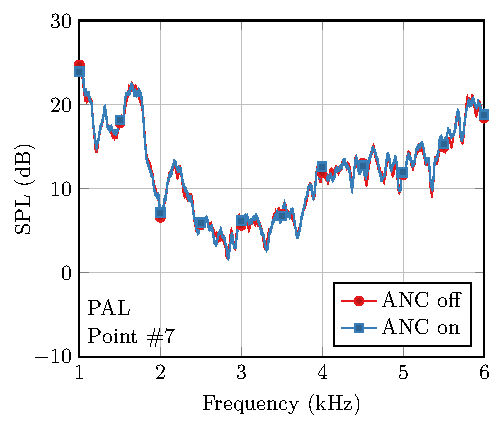
\includegraphics[width = \textwidth]{fig/PAL_eval7_ANC_spectrum.pdf}
        \caption{}
    \end{subfigure}
    \caption{SPL \revA{(dB re 20 $\mu$Pa)} at point \#2 when the secondary source was (a) a traditional loudspeaker and (b) a PAL; and at point \#7 when the secondary source was (c) a traditional loudspeaker and (d) a PAL. The distance between the secondary source and the error point was 1 m.}
    \label{fig:ancpal_compare_point27}
\end{figure}

To investigate the effects of the secondary source on the sound fields in the other areas, the SPLs at two typical evaluation points \#2 (closest to the secondary source) and \#7 (farthest away from the secondary source) with and without ANC are presented in Fig.~\ref{fig:ancpal_compare_point27}, 
where the distance between the secondary source and the error point was again 1 m. 
Both types of loudspeakers had little effect for the SPLs at point \#7 because it was away from the secondary source as shown in Figure \ref{fig:ancpal_sketch}. 
However, at point \#2 which was close to the traditional loudspeaker, the SPLs changed significantly with ANC on due to the omnidirectional secondary source, and the overall noise reduction from 1 kHz to 6 kHz of the ANC system was $\SI{-4.9}{dB}$ indicating that the overall sound energy at this point increased with ANC. 
The overall noise reduction of the ANC system using the PAL at point \#2 was only $\SI{-0.2}{dB}$ due to its sharp directivity.
Therefore, using a PAL has little effect on the sound fields in the other areas for an ANC system. 



Figure \ref{fig:ancpal_exp_overall_nr} shows the overall noise reductions from 1 kHz to 6 kHz measured by the left ear simulator of the HATS and at the 9 evaluation points with ANC on when the distance between the secondary source and the error point, which is denoted by $d\subt{se}$, was varied from 0.5 m to 3 m. 
It can be seen in Figure \ref{fig:ancpal_exp_overall_nr}(a) that the noise reductions using the PAL were similar to those when using the traditional loudspeaker, 
and are generally between 18 dB and 20 dB. 
Figure \ref{fig:ancpal_exp_overall_nr}(b) demonstrates that the noise reduction levels at all evaluation points were generally increased as the distance between the traditional loudspeaker and the error point increased. 
Figure \ref{fig:ancpal_exp_overall_nr}(c) indicates that the sound pressures at evaluation points were almost unchanged with the PAL except at points \#2 and \#5. 
The noise reduction levels at these two points were negative, indicating that the sound pressure increased with ANC on. 
The reason is that the two points were close to the radiation axis of the PAL as shown in Fig.~\ref{fig:ancpal_sketch}, and the SPL variation around them was large with and without ANC. 
The audio sound waves generated by the PAL decay slowly by distance, so the amplitude of the generated secondary sounds changes a little when the distance between the PAL and the error point increased. 
Therefore, the sound pressure in the other areas was less affected by the ANC system when the PAL was used at far away from the ear. 

\begin{figure}[!htb]
    \centering
    \begin{subfigure}{0.32\textwidth}
        \centering
        % \includegraphics[width = \textwidth]{E:/Research/InterNoise2020/matlab/exp/fig/ear_ANC_spectrum_ChangeSec.pdf}
        \includegraphics[width = \textwidth]{fig/ear_ANC_spectrum_ChangeSec.pdf}
        \caption{}
    \end{subfigure}
    \begin{subfigure}{0.32\textwidth}
        \centering
        % \includegraphics[width = \textwidth]{E:/Research/InterNoise2020/matlab/exp/fig/Genelec_ChangeSec_eval_TotalNR.pdf}
        \includegraphics[width = \textwidth]{fig/Genelec_ChangeSec_eval_TotalNR.pdf}
        \caption{}
    \end{subfigure}
    \begin{subfigure}{0.32\textwidth}
        \centering
        % \includegraphics[width = \textwidth]{E:/Research/InterNoise2020/matlab/exp/fig/PAL_ChangeSec_eval_TotalNR.pdf}
        \includegraphics[width = \textwidth]{fig/PAL_ChangeSec_eval_TotalNR.pdf}
        \caption{}
    \end{subfigure}
    \caption{Overall noise reductions from 1 kHz to 6 kHz (a) at the left ear of the HATS, and at the evaluation points, where the secondary source was (b) a traditional loudspeaker and (c) a PAL.}
    \label{fig:ancpal_exp_overall_nr}
\end{figure}


\section{Multi-channel ANC system using multiple PALs}
\label{sec:anpalqz}
In this section, the feasibility of generating a quiet zone in the free field with multiple PALs is investigated using simulations based on the SWE of the quasilinear solution of Westervelt equation as described in Sec.~\ref{sec:swe_pal}.
Both 2D and 3D configurations are investigated, where the primary sources are assumed to be point monopoles located randomly on a two-dimensional plane, or in three-dimensional space. 
For a 2D problem, the secondary sources are uniformly distributed around the circumference of a circle on the same plane of primary sources. 
For a 3D problem, the secondary sources are uniformly distributed over a spherical surface. 
The relationship between the sound wavelength, the number of secondary sources, and the size of the quiet zone generated by the PALs is explored, and the influence of PALs on the sound field outside the quiet zone is discussed. 
Numerical simulations are also validated against experimental data.
\subsection{Theory}
Figures \ref{fig:ancpal:sketch2d} and \ref{fig:ancpal:sketch3d} show the schematic diagram of the ANC system to be investigated. 
The primary sources consist of $N\subt{p}$ point monopoles randomly located on the $xOy$ plane, or in three-dimensional space. 
They are assumed to be harmonic with frequency $f$. 
The number of secondary sources is $N\subt{s}$, and they are uniformly distributed on a circle on the $xOy$ plane, or a sphere with a radius of $R\subt{s}$, as shown in Figs. \ref{fig:ancpal:sketch2d} and \ref{fig:ancpal:sketch3d}, respectively. 
For all cases, the target zone to be controlled is a two-dimensional interior region of a circle on the $xOy$ plane with a radius of $R_0$ centered at the origin of the rectangular coordinate system $Oxyz$.
\begin{figure}[!htb]
    \centering
    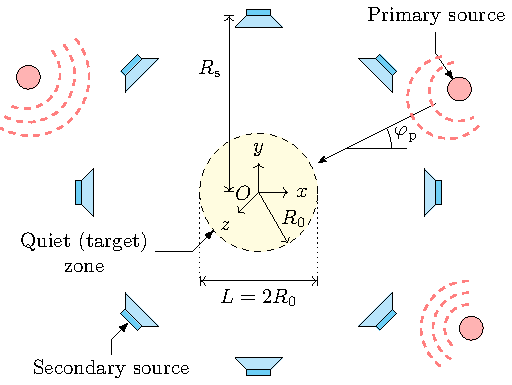
\includegraphics[width = 0.6\textwidth]{fig/sketch_v5.pdf}
    \caption{Sketch of an ANC system where the primary and secondary sources are located on the $xOy$ plane. }
    \label{fig:ancpal:sketch2d}
\end{figure}

\begin{figure}[!htb]
    \centering
    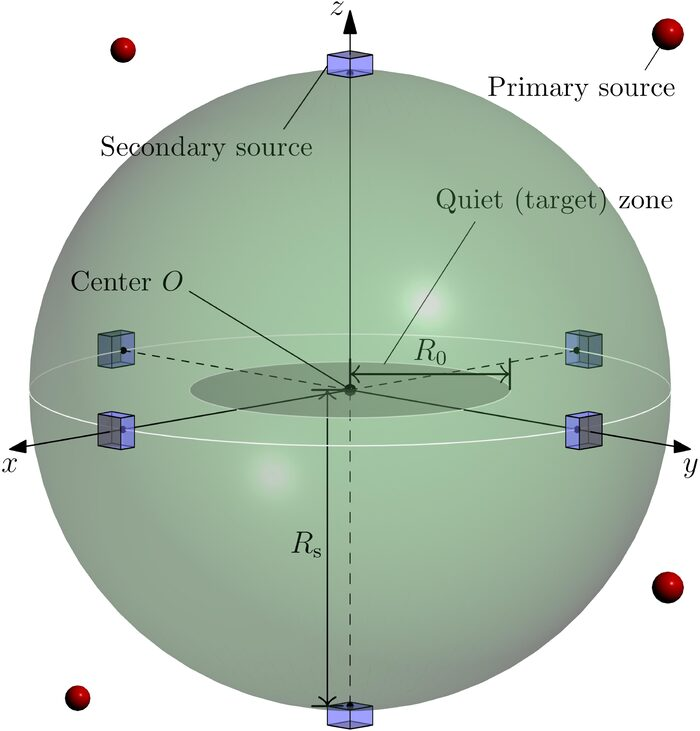
\includegraphics[width = 0.4\textwidth]{fig/ANC3D_resize.jpg}
    \caption{Sketch of an ANC system where the primary and secondary sources are located in three-dimensional space.}
    \label{fig:ancpal:sketch3d}
\end{figure}


The summation of the square of the sound pressure at each error point is chosen as the cost function for the ANC system, which yields \cite{Kirkeby1996LocalSoundField, Qiu2019IntroductionVirtualSound}
\begin{equation}
    \calJ  = 
    \vb{p}\subt{et}^\rmH\vb{p}\subt{et}
    +
    \beta_0 \vb{Q}\subt{s}^\rmH \vb{Q}\subt{s}
\end{equation}
where $\vb{p}\subt{ep}$ and $\vb{p}\subt{es}$ are the sound pressure vectors at error points radiated by primary and secondary sources, respectively, and $\vb{p}\subt{et} = \vb{p}\subt{ep} + \vb{p}\subt{es}$. 
In addition, $\beta_0$ is a real number to constrain the outputs of secondary sources \cite{Kirkeby1996LocalSoundField}, $\vb{Q}\subt{s}$ is the source strength vector of the secondary sources, and the superscripts \quotes{T} and \quotes{H} denote the transpose and the conjugate transpose, respectively. 
The optimized source strengths of the secondary sources are \cite{Qiu2019IntroductionVirtualSound}
\begin{equation}
    % 2
    \vb{Q}\subt{s,opt}
    = 
    -(\vb{Z}\subt{es}^\rmH \vb{Z}\subt{es} + \beta_0 \vb{I} )^{-1}
    \vb{Z}\subt{es}^\rmH
    \vb{p}\subt{ep}
\end{equation}
where $\vb{Z}\subt{es}$ is a matrix of the acoustic transfer functions from $N\subt{s}$ secondary sources to $N\subt{e}$ error points, and $\vb{I}$ is an identity matrix of size $N\subt{s}$. 
After obtaining the optimal secondary source strengths, the total sound pressure with control can be calculated. 

In this section, both traditional omnidirectional loudspeakers and PALs are adopted as secondary sources. 
The traditional loudspeakers are modeled as point monopoles, where the sound pressure is given as
\begin{equation}
    p(\vb{r})
    =-\rmi \rho_0\omega Q_0
    \frac{\rme^{\rmi k \abs{\vb{r}-\vb{r}_0}}}{4\uppi\abs{\vb{r}-\vb{r}_0}}
    \label{eq:ancpal:32980fjs}
\end{equation}
where $\rho_0$ is the air density, $\omega = 2\uppi f$ is the angular frequency, $k = \omega/c_0$ is the wavenumber, $Q_0$ is the source strength, and $\abs{\vb{r}-\vb{r}_0}$ is the distance between the field point $\vb{r}$ and the source point $\vb{r}_0$. 

The audio sound pressure radiated by a PAL can be considered as a superposition of the pressure radiated by infinite virtual sources in air with the source density function proportional to the sound pressure of ultrasound. 
This can be calculated as
\begin{equation}
    % 4
    p(\vb{r}, k)
    =
    -\rmi \rho_0\omega
    u_1u_2^* 
    \iiint_V
    q(\vb{r}\subt{v})
    \frac{\rme^{\rmi k \abs{\vb{r}-\vb{r}\subt{v}}}}{4\uppi \abs{\vb{r}-\vb{r}\subt{v}}}
    \dd^3 \vb{r}\subt{v}
\end{equation}
where $u_1$ and $u_2$ are the amplitude of the vibration velocity on the transducer surface for the ultrasound $f_1$ and $f_2$ ($f_1 > f_2$), respectively. 
Furthermore, the PAL is assumed to be placed at the origin and radiates in the positive axial direction, where the superscript \quotes{*} denotes the complex conjugate, the integration range $V$ represents the whole three-dimensional space, and $q(\vb{r}\subt{v})$ is the source density function at the virtual source point $\vb{r}\subt{v}$ determined by the ultrasound pressure. 
The radiated audio sound pressure can be tuned by controlling the values of $u_1$ and $u_2$ of the ultrasound, so that $u_1u_2^*$ is defined as the source strength of a PAL, which is equivalent to $Q_0$ in Eq.~(\ref{eq:ancpal:32980fjs}).

To investigate the performance of the ANC system, the sound pressure in a large square region with dimensions of $\SI{-2}{m} \leq x \leq \SI{2}{m}$, and $\SI{-2}{m}\leq y \leq \SI{2}{m}$ and its center at the origin $O$, is calculated for all cases. 
A mesh of squares in this region is generated with a separation between grid points no larger than 1/20 of wavelength. 
All grid points are chosen as evaluation points, while only the ones inside the circular target zone are chosen as the error points. 

The noise reduction (NR) inside the circular target zone is defined as
\begin{equation}
    % 5
    \rmNR 
    =
    10\log_{10}
    \qty(\frac{\vb{p}\subt{ep}^\rmH \vb{p}\subt{ep}}{\vb{p}\subt{et}^\rmH \vb{p}\subt{et}})
    \quad
    \qty(\rmdB)
\end{equation}
NR decreases as the radius of the circular target zone increases, so that the size of the quiet zone $L$ is defined as the diameter of the maximal target zone satisfying that the NR is greater than 10 dB. 

To evaluate the spillover effect of secondary sources on the surrounding areas quantitatively, a measure called \quotes{energy gain} is defined as
\begin{equation}
    % 6
    G = 
    10\log_{10}
    \qty(\frac{\vb{p}\subt{vt}^\rmH \vb{p}\subt{vt}}{\vb{p}\subt{vp}^\rmH \vb{p}\subt{vp}})
    \quad
    \qty(\rmdB)
\end{equation}
where $\vb{p}\subt{vp}$ and $\vb{p}\subt{vs}$ are the sound pressure vectors at evaluation points radiated by primary and secondary sources, respectively, and $\vb{p}\subt{vt} = \vb{p}\subt{vp} + \vb{p}\subt{vs}$. 
The result $G < 0$ indicates the total acoustic energy in the square region is reduced, while $G > 0$ shows that that the total acoustic energy increases in the square region even though a smaller quiet zone is generated at its center.

\subsection{Simulations}
Two configurations of secondary sources are considered in this section. 
The two-dimensional configuration denoted by \quotes{2D secondary source array} is shown in Fig.~\ref{fig:ancpal:sketch2d} where $N\subt{s}$ secondary sources ($N\subt{s} = 8$ in the figure) are evenly placed on a circle and the azimuthal angle at the $i$\mbox{-th} source is $\varphi_{\rms, i} = 2\uppi(i-1)/N\subt{s}$, $i = 1, 2, …, N\subt{s}$. 
The three-dimensional configuration denoted by \quotes{3D secondary source array} is shown in Fig.~\ref{fig:ancpal:sketch3d}, where $N\subt{s}$ secondary sources ($N\subt{s} = 6$ in the figure) are evenly placed on a spherical surface and the minimal distance between arbitrary two secondary sources is denoted by $d\subt{min}$. 
The secondary source locations are obtained by maximizing $d\subt{min}$, and the source coordinates for different $N\subt{s}$ can be found in \cite{SloaneSphericalCodesNice}. 
The radius of the secondary source array is set to be $R\subt{s} = \SI{1.5}{m}$ in all of the simulations that follow.

The quiet zone size, $L$, is obtained by using an iterative procedure. 
The initial lower ($R_1$) and upper ($R_2$) values are set to 0 and 1.5 m, respectively. 
The NR inside the circular target zone is calculated when the radius of the target zone $R_0$ is set as $(R_1 + R_2)/2$. 
If $\rmNR < \SI{10}{dB}$, the upper value $R_2$ is updated as $(R_1 + R_2)/2$. 
If $\rmNR > \SI{10}{dB}$, the lower value $R_1$ is updated as $(R_1 + R_2)/2$. 
The iteration stops when $(R_2 – R_1)$ is less than 1/20 of the wavelength and $(R_1 + R_2)$ is chosen as the quiet zone size $L$. 
All simulation results presented here have followed this procedure. 
Each PAL is assumed to be circular with a radius of 0.1 m and a uniform surface velocity profile for the ultrasound. 
The lower ultrasound frequency is set as 64 kHz, which is a typical carrier frequency for commercial PALs \cite{HolosonicsAudioSpotlight24i}.
The sound attenuation coefficients at both ultrasonic and audio sound frequencies are calculated according to ISO 9613-1 with a relative humidity of 60\% and a temperature of $25\celsius$. 
The audio sound generated by each PAL is calculated using the spherical expansion method proposed in Sec.~\ref{sec:swe_pal}.

\subsubsection{2D secondary source array}
\label{sec:ancpalqz_2d}
Figure \ref{fig:ancpalqz:2d:compare} shows the primary and total sound fields at 1 kHz under the optimal control by 8 PALs, or point monopoles, shown as black rectangles or circles, respectively, where the primary source (not shown in the figure) is a single monopole located at an azimuthal angle of $\varphi\subt{p} = 22.5^\circ$ with a distance to the origin of 4 m. 
The angle of $22.5^\circ$ is selected because it is the angle of the bisector of the first and second secondary sources, which is the worst case for the NR performance \cite{Qiu2019IntroductionVirtualSound}.
The quiet zone size in Figs. \ref{fig:ancpalqz:2d:compare}(b) and (c) is 0.45 m and 0.46 m, respectively. 
Although the quiet zone sizes are similar, the energy gain associated with the point monopole sources is 6.9 dB, which is much larger than the $\SI{-0.1}{dB}$ obtained with the PALs. 
The decrement of energy is mainly contributed from the noise reduction in the quiet zone, and it is roughly same for both kinds of loudspeakers. 
The sound pressure around the traditional loudspeakers located on the direction of the primary source is large, so that the noise amplification can be clearly observed. 
However, it is not observed when using PALs because they generate unidirectional secondary waves and these waves decay slowly along the propagation path. 
This is the reason the energy gain when using PALs is much smaller than that using traditional loudspeakers. 

\begin{figure}[!htb]
    \centering
    \begin{subfigure}{0.32\textwidth}
        \centering
        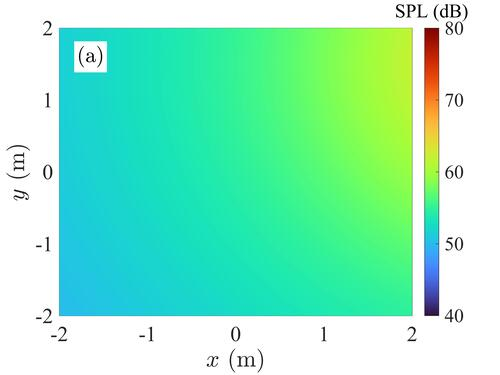
\includegraphics[width = \textwidth]{fig/cal_ANC_QuietZone_demo_pri_200503B_resize.jpg}
    \end{subfigure}
    \begin{subfigure}{0.32\textwidth}
        \centering
        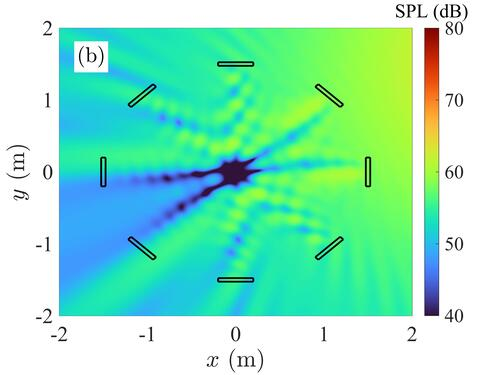
\includegraphics[width = \textwidth]{fig/cal_ANC_QuietZone_demo_tot_PAL_200503B_resize.jpg}
    \end{subfigure}
    \begin{subfigure}{0.32\textwidth}
        \centering
        % \includegraphics[width = \textwidth]{E:/Research/Archive/PalAncQuietZone2003/matlab/anc/fig/cal_ANC_QuietZone_demo_tot_Monopole_200503B_resize.jpg}
        \includegraphics[width = \textwidth]{fig/cal_ANC_QuietZone_demo_tot_Monopole_200503B_resize.jpg}
    \end{subfigure}
    \caption{Audio \revA{SPL (dB re 20 $\mu$Pa)} at 1 kHz (a) for the primary noise comes from the direction $\varphi_{\mathrm{p} }= 22.5^\circ$, (b) under the optimal control with 8 PALs, and (c) under the optimal control with 8 point monopoles.}
    \label{fig:ancpalqz:2d:compare}
\end{figure}


Figure \ref{fig:ancpalqz:diff_num_sec} shows the quiet zone size and energy gain as a function of the azimuthal angle of a primary source 4 m away from the origin at 1 kHz for various numbers of secondary sources. 
The peaks and valleys in Fig.~\ref{fig:ancpalqz:diff_num_sec} (a) and (b) are associated with the location of the secondary sources. 
It is clear that the quiet zone size increases when the primary wave angle approaches that of the secondary source, which is due to better matching of the wave fronts from the primary and secondary sound waves \cite{Guo1997ActivelyCreatedQuiet}.
In most cases when there is one secondary source, the difference between the size of the quiet zone for the PAL and the point monopole secondary sources is less than 10\% when the primary source angle is greater than $20^\circ$. 
The minimal quiet zone size is also 0.035 m when the primary source angle is at $180^\circ$, and the size is about a tenth of the wavelength. 

\begin{figure}[!htb]
    \centering
    \begin{subfigure}{0.49\textwidth}
        \centering
        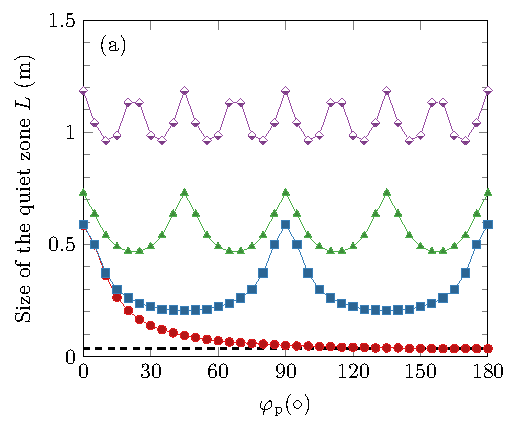
\includegraphics[width = \textwidth]{fig/200325K_size_PAL_v3.pdf}
    \end{subfigure}
    \begin{subfigure}{0.49\textwidth}
        \centering
        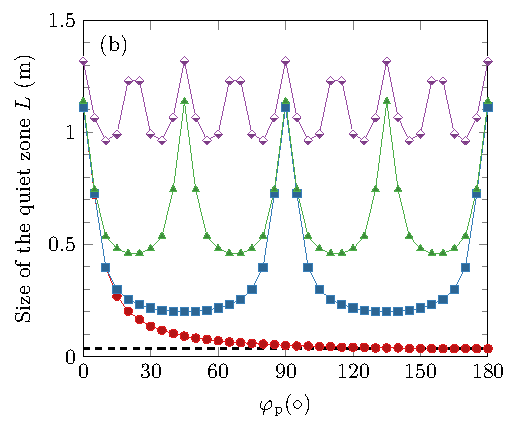
\includegraphics[width = \textwidth]{fig/200325K_size_Monopole_v3.pdf}
    \end{subfigure}
    \\
    \begin{subfigure}{0.49\textwidth}
        \centering
        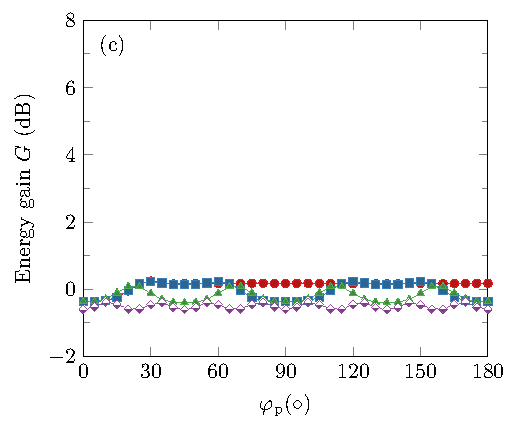
\includegraphics[width = \textwidth]{fig/200325K_gain_PAL_v2.pdf}
    \end{subfigure}
    \begin{subfigure}{0.49\textwidth}
        \centering
        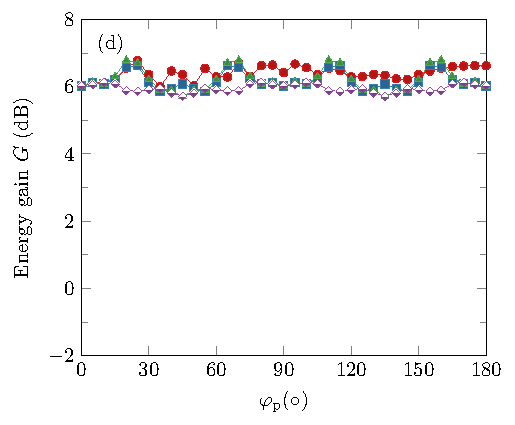
\includegraphics[width = \textwidth]{fig/200325K_gain_Monopole_v2.pdf}
    \end{subfigure}
    \caption{The quiet zone size and energy gain as a function of the primary source azimuthal angles at 1 kHz for different numbers of secondary sources: (a) and (b) the quiet zone size created by PALs and point monopoles, respectively; (c) and (d) the energy gain caused by PALs and point monopoles, respectively. Red circles, $N\subt{s} = 1$; blue squares, $N\subt{s} = 4$; green triangles, $N\subt{s} = 8$; purple diamonds, $N\subt{s} = 16$; dashed line, $\lambda/10$.}
    \label{fig:ancpalqz:diff_num_sec}
\end{figure}

It is shown in Fig.~\ref{fig:ancpalqz:diff_num_sec} that increasing secondary source number enlarges the size of the quiet zone. 
For example, the minimal quiet zone size is 0.035 m, 0.2 m, 0.46 m, and 0.97 m when the secondary source number is 1, 4, 8, and 16, respectively. 
The primary source azimuthal angles with minimal quiet zone sizes are the ones with their bisector between two adjacent secondary sources. 
Although the quiet zone size created by both PAL and point monopole secondary sources are approximately the same in most cases, 
the energy gain caused by the point monopoles are generally above 6 dB which is larger than the one caused by PALs which is around 0 dB.

To understand the performance of the ANC systems under complex acoustic environments, in the next examples 8 primary sources are placed on the same plane {as} the secondary source array, where the distance between each primary source and the origin is randomly and uniformly set between 3.5 m and 4.5 m; 
the azimuthal angle is randomly and uniformly set between 0 and $360^\circ$; 
the source strength is randomly and uniformly set between $\SI{0.75e-4}{m^3/s}$ and $\SI{1.25e-4}{m^3/s}$; 
and this configuration is denoted here as \quotes{2D primary sound field}. 
Figure \ref{fig:ancpalqz:2d:rand:compare} shows the results of one trial of the 2D primary sound field and the total sound field controlled by 8 secondary sources. 
The quiet zone size created by both sources is 0.53 m, while the energy gain is $\SI{-0.2}{dB}$ with the PALs, and 6.5 dB with the point monopoles. 

\begin{figure}[!htb]
    \centering
    \begin{subfigure}{0.32\textwidth}
        \centering
        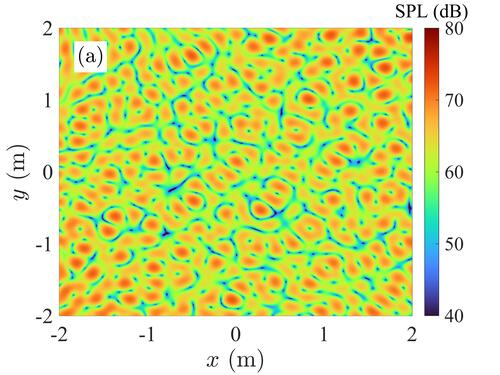
\includegraphics[width = \textwidth]{fig/cal_ANC_QuietZone_demo_pri_200503C_resize.jpg}
    \end{subfigure}
    \begin{subfigure}{0.32\textwidth}
        \centering
        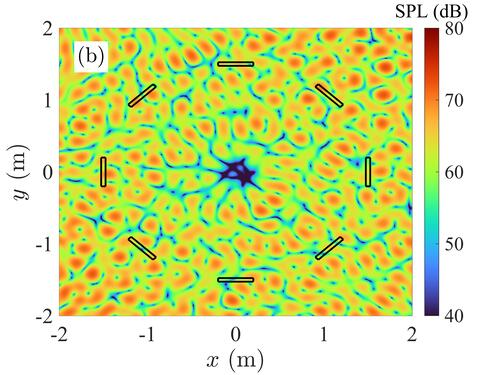
\includegraphics[width = \textwidth]{fig/cal_ANC_QuietZone_demo_tot_PAL_200503C_resize.jpg}
    \end{subfigure}
    \begin{subfigure}{0.32\textwidth}
        \centering
        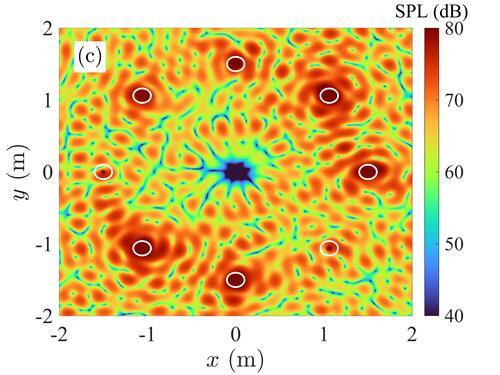
\includegraphics[width = \textwidth]{fig/cal_ANC_QuietZone_demo_tot_Monopole_200503C_resize.jpg}
    \end{subfigure}
    \caption{Audio \revA{SPL (dB re 20 $\mu$Pa)} at 1 kHz (a) generated by 8 point monopoles randomly located on the $xOy$ plane, (b) under the optimal control with 8 PALs, and (c) under the optimal control with 8 point monopoles.}
    \label{fig:ancpalqz:2d:rand:compare}
\end{figure}

Figure \ref{fig:ancpalqz:rand:qz_eg} shows the quiet zone size and energy gain based on 100 trials of random 2D primary sound fields generated by 8 point monopoles randomly located on the $xOy$ plane. 
The quiet zone size decreases as the frequency increases in all cases and is about $0.75\lambda, 1.5\lambda$, and $3\lambda$ under optimal control conditions with 4, 8, and 16 point monopoles, respectively, 
where $\lambda$ is the wavelength of the sound at the corresponding frequency. 
The quiet zone size generated by point monopoles is larger than the one generated by PALs especially at the low frequencies; however, the difference between them becomes negligible at the middle and high frequencies. 
For example, the quiet zone sizes are 1.33 m and 1.21 m respectively for 8 monopoles and PALs at 400 Hz, while both become about 0.55 m at 1 kHz. 
The energy gain caused by the point monopoles is always larger than the one caused by the PALs, which is seen to increase only slightly as the frequency increases.

\begin{figure}[!htb]
    \centering
    \begin{subfigure}{0.32\textwidth}
        \centering
        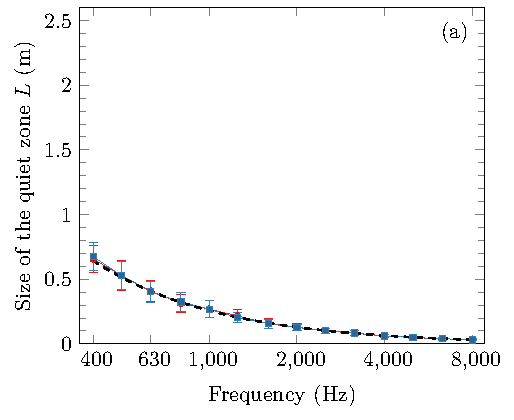
\includegraphics[width = \textwidth]{fig/200404A_size_v2}
    \end{subfigure}
    \begin{subfigure}{0.32\textwidth}
        \centering
        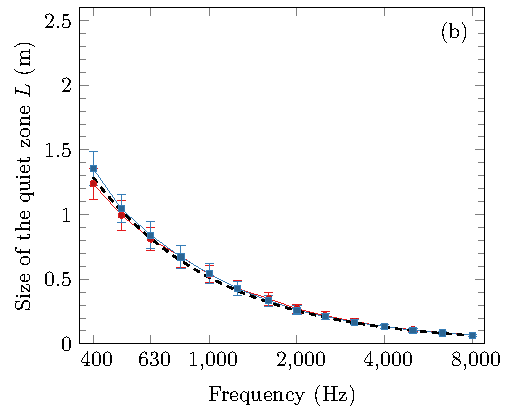
\includegraphics[width = \textwidth]{fig/200331A_size_v2}
    \end{subfigure}
    \begin{subfigure}{0.32\textwidth}
        \centering
        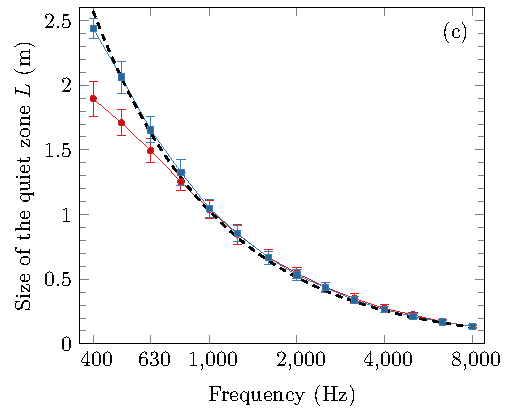
\includegraphics[width = \textwidth]{fig/200404B_size_v2}
    \end{subfigure}
    \\
    \begin{subfigure}{0.32\textwidth}
        \centering
        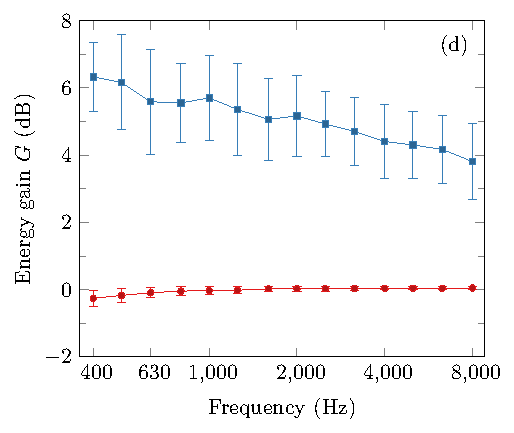
\includegraphics[width = \textwidth]{fig/200404A_gain_v2}
    \end{subfigure}
    \begin{subfigure}{0.32\textwidth}
        \centering
        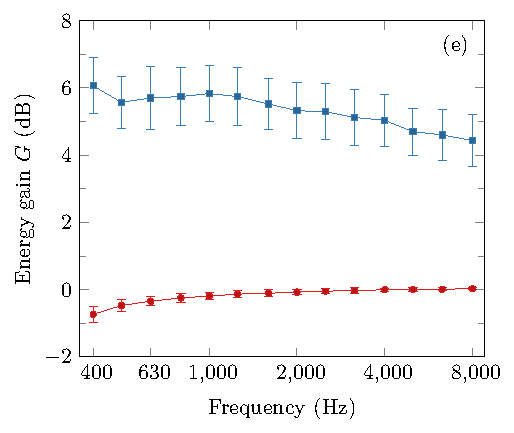
\includegraphics[width = \textwidth]{fig/200331A_gain_v2}
    \end{subfigure}
    \begin{subfigure}{0.32\textwidth}
        \centering
        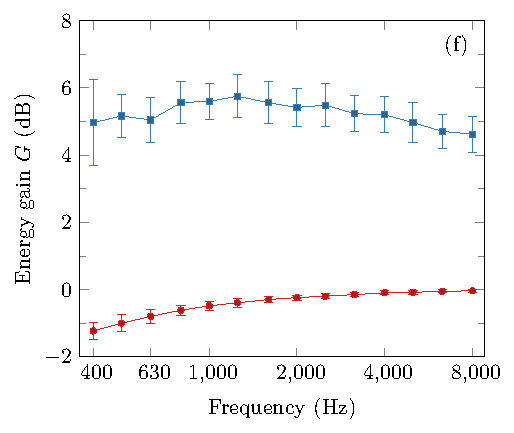
\includegraphics[width = \textwidth]{fig/200404B_gain_v2}
    \end{subfigure}
    \caption{For random 2D primary sound fields under the optimal control with the 2D secondary sources, (a), (b), and (c) the quiet zone size when the secondary source number is 4, 8, and 16, respectively; (d), (e), and (f) the energy gain when the secondary source number is $N\subt{s} = 4, 8$, and 16, respectively, where the value and error bar are the mean value and standard deviation of 100 random trials, and $\lambda$ is the wavelength. Red circles, PAL; blue squares, monopole; dashed lines, $0.75\lambda$, $1.5\lambda$, and $3\lambda$ for (a), (b), and (c), respectively.}
    \label{fig:ancpalqz:rand:qz_eg}
\end{figure}

Figure \ref{fig:ancpalqz:qz_eg:rand:2d} shows the quiet zone size and energy gain at different numbers of secondary sources at 1 kHz and 2 kHz. 
It is clear the quiet zone size increases as the number of secondary sources increases. 
When the secondary source number becomes large, the quiet zone size increases slowly due to the limitations of the size of secondary source array (3 m) and the narrow beam width of sound radiated by PALs. 
As shown in Fig.~\ref{fig:ancpalqz:qz_eg:rand:2d}(a), when the secondary source number is, respectively, less than 20 and 48 at 1 kHz and 2 kHz, the quiet zone size is approximately proportional to the secondary source number and can be estimated by the following formula 

\begin{equation}
    % 7
    L = 0.19\lambda N\subt{s}
    \label{eq:ancpalqz:L19N}
\end{equation}
For the ANC systems with $N\subt{s}$ secondary sources, the arc length between adjacent secondary sources can be obtained by dividing the circumference of the generated quiet zone to give a length of $\uppi L / N\subt{s} $. 
Using the $L$ value in Eq.~(\ref{eq:ancpalqz:L19N}), the arc length is about $0.6\lambda$ which indicates that the separation between secondary sources is about one half of the wavelength. 
This agrees with the remarks in \cite{Qiu2019IntroductionVirtualSound} and \cite{Nelson1992ActiveControlSound}.
Figure \ref{fig:ancpalqz:qz_eg:rand:2d}(b) indicates that the energy gain can also be reduced by introducing more secondary sources and the reduction is more significant at lower frequencies.

\begin{figure}[!htb]
    \centering
    \begin{subfigure}{0.49\textwidth}
        \centering
        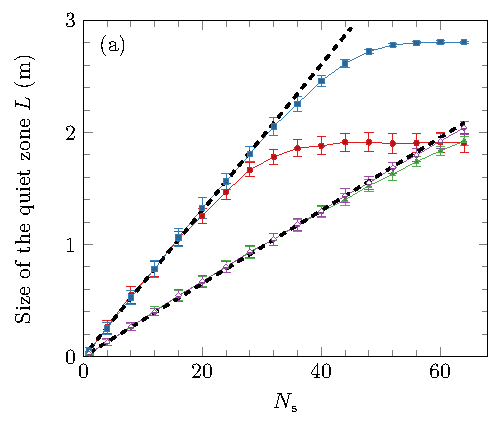
\includegraphics[width = \textwidth]{fig/200407A_size_v2.pdf}
    \end{subfigure}
    \begin{subfigure}{0.49\textwidth}
        \centering
        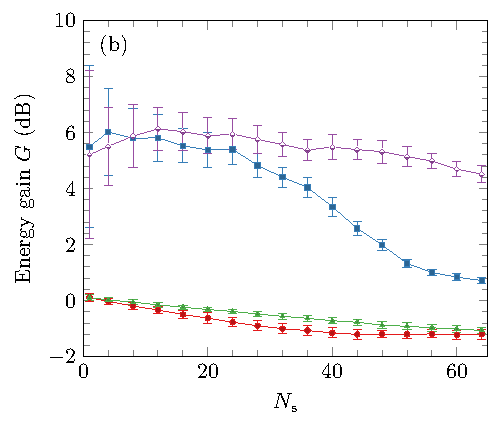
\includegraphics[width = \textwidth]{fig/200407A_gain_v2.pdf}
    \end{subfigure}
    \caption{For random 2D primary sound fields under the optimal control with 2D secondary sources at 1 kHz and 2 kHz: (a) the quiet zone size as a function of secondary source number; (b) the energy gain as a function of secondary source number. Red circles, PAL at 1 kHz; blue squares, monopole at 1 kHz; green triangles, PAL at 2 kHz; purple diamonds, monopole at 2 kHz.}
    \label{fig:ancpalqz:qz_eg:rand:2d}
\end{figure}

In the following simulations, the primary noise comes from multiple directions in three-dimensional space and the configuration is denoted by \quotes{3D primary sound field}, 
although the secondary sources are still located on the two-dimensional $xOy$ plane. 
Figure \ref{fig:ancpalqz:qz_eg:rand:2d2} shows the quiet zone size and energy gain based on 100 random trials of 3D primary sound fields under the optimal control of 8 secondary sources in the $xOy$ plane. 
Compared with Fig.~\ref{fig:ancpalqz:rand:qz_eg}(b), the mean value of the quiet zone size decreases from $1.5\lambda$ to $0.75\lambda$, 
while the standard deviation shows no significant changes. 
Compared with Fig.~\ref{fig:ancpalqz:rand:qz_eg}(e), the energy gain caused by the PALs becomes positive at most frequencies, while it is still much less than the one caused by the point monopoles.

\begin{figure}[!htb]
    \centering
    \begin{subfigure}{0.49\textwidth}
        \centering
        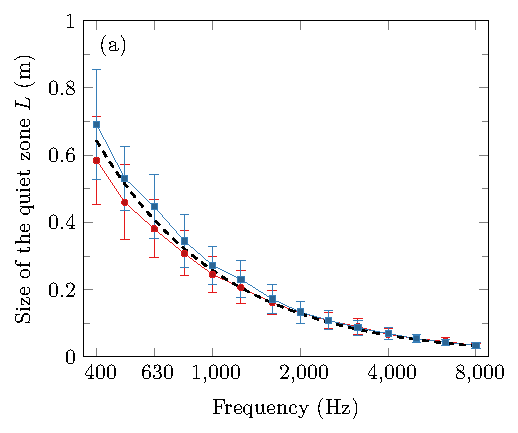
\includegraphics[width = \textwidth]{fig/200405A_size_v2}
    \end{subfigure}
    \begin{subfigure}{0.49\textwidth}
        \centering
        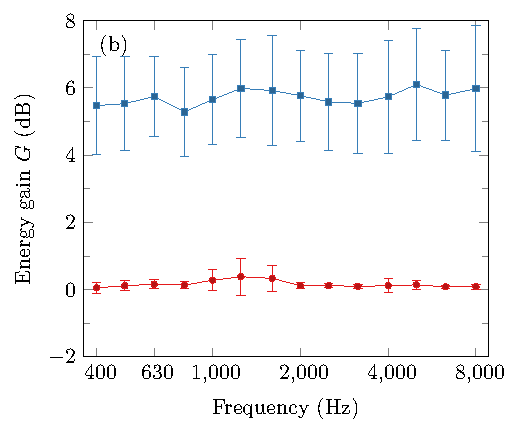
\includegraphics[width = \textwidth]{fig/200405A_gain_v2}
    \end{subfigure}
    \caption{For random 3D primary sound fields under the optimal control with eight 2D secondary sources in the plane $xOy$, (a) the quiet zone size as a function of frequency; (b) the energy gain as a function of frequency. Red circles, PAL; blue squares, monopole; dashed line, $0.75\lambda$.}
    \label{fig:ancpalqz:qz_eg:rand:2d2}
\end{figure}

Figure \ref{fig:ancpalqz:qz_eg:rand:3dpri:2dsec} shows the quiet zone size and energy gain based on 100 random trials of 3D primary sound fields using different numbers of 2D secondary sources. 
When the secondary source number $N\subt{s}$ is small, the quiet zone size increases as $N\subt{s}$ increases, but it changes slightly when $N\subt{s} > 10$. 
At 1 kHz, the quiet zone size generated by using the point monopoles and PALs approaches 0.29 m and 0.27 m, respectively, at large secondary source numbers. 
At 2 kHz, the quiet zone size approaches to 0.14 m. 
The maximal quiet zone size is about $0.75\lambda$ no matter how many secondary sources are used. 
When $N\subt{s} < 8$, the quiet zone size can be estimated as 
\begin{equation}
    % 8
    L =0.095\lambda N\subt{s}
\end{equation}
which is a half of that in Eq.~(\ref{eq:ancpalqz:L19N}). 
The reason for having a small quiet zone size is that the primary noises coming out of the xOy plane cannot be effectively controlled due to that fact that no secondary sources are placed in these directions. 
Furthermore, the energy gain caused by both types of secondary sources decreases with an increasing number of secondary sources, as shown in Fig.~\ref{fig:ancpalqz:qz_eg:rand:3dpri:2dsec}(b).

\begin{figure}[!htb]
    \centering
    \begin{subfigure}{0.49\textwidth}
        \centering
        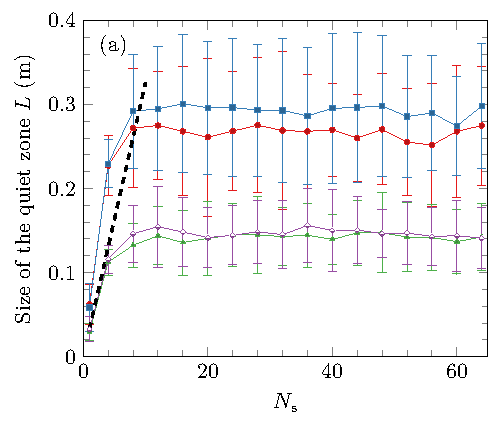
\includegraphics[width = \textwidth]{fig/200410A_size_v2}
    \end{subfigure}
    \begin{subfigure}{0.49\textwidth}
        \centering
        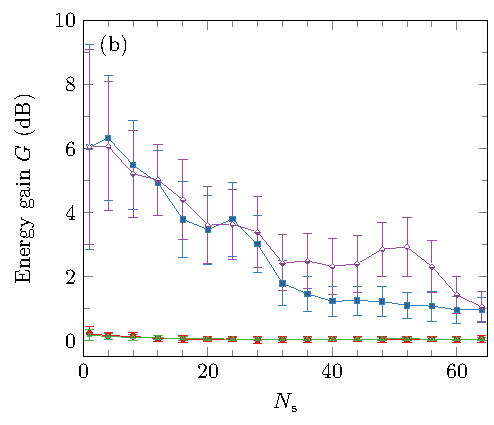
\includegraphics[width = \textwidth]{fig/200410A_gain_v2}
    \end{subfigure}
    \caption{For random 3D primary sound fields controlled by 2D secondary sources at 1 kHz and 2 kHz: (a) the quiet zone size as a function of secondary source number; (b) the energy gain as a function of secondary source number. Red circles, PAL at 1 kHz; blue squares, monopole at 1 kHz; green triangles, PAL at 2 kHz; purple diamonds, monopole at 2 kHz; dashed line, $0.095\lambda N\subt{s}$.}
    \label{fig:ancpalqz:qz_eg:rand:3dpri:2dsec}
\end{figure}

\subsubsection{3D secondary source array}

Figure \ref{fig:ancpalqz_3dpri_3dsec} shows the quiet zone size and energy gain when random 3D primary sound fields are optimally controlled by 8 and 20 secondary sources located in three-dimensional space at different frequencies. 
Compared with Fig.~\ref{fig:ancpalqz:qz_eg:rand:2d2}(a), the quiet zone size increases from $0.75\lambda$ to $\lambda$ by using a 3D instead of 2D secondary source array, even with the same number of secondary sources ($N\subt{s} = 8$). 
Therefore, the quiet zone size is not limited by $0.75\lambda$, as was the case for 2D secondary sources, but may be increased to $2.2\lambda$ when the secondary source number is 20. 
For the monopoles, although the quiet zone is enlarged, the energy gain is also increased, this time by more than 2-4 dB as the number of secondary sources increased from 8 to 20 as shown in Fig.~\ref{fig:ancpalqz_3dpri_3dsec}(b).

\begin{figure}[!htb]
    \centering
    \begin{subfigure}{0.49\textwidth}
        \centering
        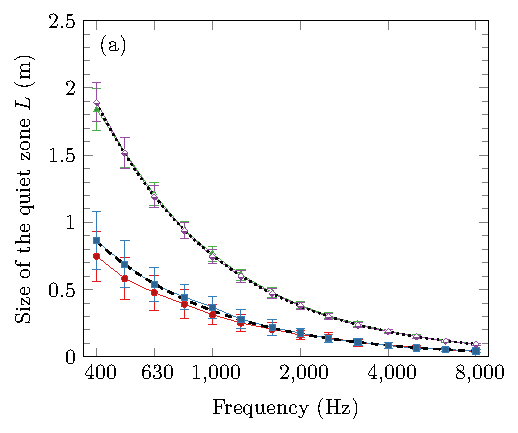
\includegraphics[width = \textwidth]{fig/200409A_size_v2}
    \end{subfigure}
    \begin{subfigure}{0.49\textwidth}
        \centering
        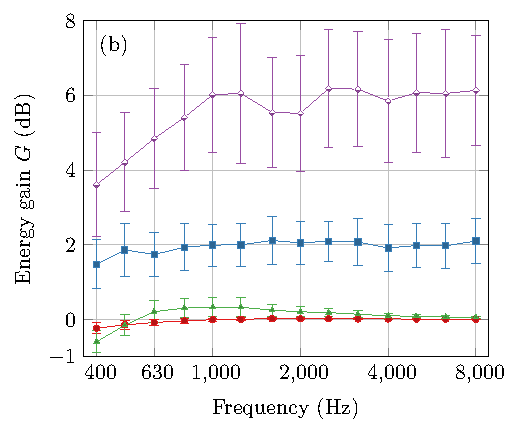
\includegraphics[width = \textwidth]{fig/200409A_gain_v3}
    \end{subfigure}
    \caption{For random 3D primary sound fields under the optimal control with the 3D secondary sources, (a) the quiet zone size as a function of frequency; (b) the energy gain as a function of frequency. 
    Red circles, PAL when $N\subt{s} = 8$; blue squares, monopole when $N\subt{s} = 8$; green triangles, PAL when $N\subt{s} = 20$; purple diamonds, monopole when $N\subt{s} = 20$; dashed line, $\lambda$; dotted line, $2.2\lambda$.}
    \label{fig:ancpalqz_3dpri_3dsec}
\end{figure}

Figure \ref{fig:ancpalqz_3dpri_3dsec_vary_secnum} shows the quiet zone size and energy gain when random 3D primary sound fields are optimally controlled by the 3D secondary source array at 1 kHz and 2 kHz. 
The quiet zone size is observed to be approximately proportional to the square root of the secondary source number, and can be estimated by
\begin{equation}
    L = 0.55\lambda \sqrt{N\subt{s}}
    % 9
    \label{eq:ancpalqz_055N}
\end{equation}
at all cases when the secondary source number $N\subt{s}$ is less than 120. 
To control the 3D primary sound field, the secondary sources are distributed evenly on a spherical surface. 
Suppose there is a smaller sphere with a diameter of $L$ centered at the origin and enclosed by the secondary source array. 
The area of this sphere divided by $N\subt{s}$ is $\uppi L^2/N\subt{s}$, and by using the value for $L$ from Eq.~(\ref{eq:ancpalqz_055N}), 
the area that can be controlled by each secondary source is then $0.95\lambda^2$. 
In other words, the size of the area controlled by each secondary source is about one wavelength. 
As for the energy gain, the gain from using the monopoles varies significantly at different secondary source numbers, whereas the gain from the PALs is much smaller for both the mean value and standard deviation.

\begin{figure}[!htb]
    \centering
    \begin{subfigure}{0.49\textwidth}
        \centering
        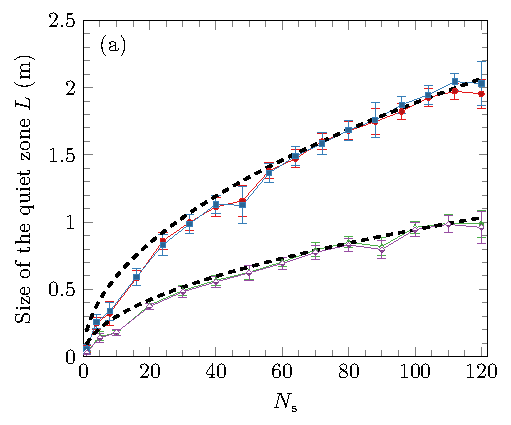
\includegraphics[width = \textwidth]{fig/200408A_size_v2}
    \end{subfigure}
    \begin{subfigure}{0.49\textwidth}
        \centering
        \includegraphics[width = \textwidth]{fig/200408A_gain_v3}
    \end{subfigure}
    \caption{For random 3D primary sound fields under the optimal control with the 3D secondary sources, (a) the quiet zone size as a function of secondary source number; (b) the energy gain as a function of secondary source number. Red circles, PAL at 1 kHz; blue squares, monopole at 1 kHz; green triangles, PAL at 2 kHz; purple diamonds, monopole at 2 kHz; dashed line, $0.55\lambda\sqrt{N\subt{s}}$.}
    \label{fig:ancpalqz_3dpri_3dsec_vary_secnum}
\end{figure}

\subsection{Experiments}
The experiments were conducted in a full anechoic room at Nanjing University with dimensions of $\SI{11.4}{m} \times \SI{7.8}{m} \times\SI{6.7}{m}$ (height). 
The sketch and photo of the experimental setup and equipment are shown in Figs. \ref{fig:ancpalqz_exp_sketch} and \ref{fig:ancpalqz_exp_photo}, respectively. 
All equipment was placed at the same height. 
Four commercial PALs (Audio Spotlight AS-16i, Holosonics \cite{HolosonicsAudioSpotlight24i}) were used and evenly located on a circle with a radius of 2.2 m, which is a 2D configuration with 4 secondary sources, as discussed in Sec.~\ref{sec:ancpalqz_2d}. 
The PAL has a surface size of $\SI{0.4}{m} \times \SI{ 0.4}{m}$ and a carrier frequency of 64 kHz. 
Four laboratory made traditional loudspeakers with dimensions of $\SI{20.7}{ cm} \times \SI{18.7}{cm }\times\SI{ 11.6}{cm}$ were used as primary sources and they were placed on a circle with a radius of 2.5 m. 

\begin{figure}[!htb]
    \centering
    \includegraphics[width = 0.8\textwidth]{fig/exp_setup_v1.pdf}
    \caption{ Top view of the experiment setup in a full anechoic room.}
    \label{fig:ancpalqz_exp_sketch}
\end{figure}

\begin{figure}[!htb]
    \centering
    \includegraphics[width = 0.5\textwidth]{fig/exp_setup_v3_resize.png}
    \caption{Photo of the experiment setup in a full anechoic room.}
    \label{fig:ancpalqz_exp_photo}
\end{figure}

An error microphone array was placed at the center with a size of $\SI{0.55}{m}\times \SI{0.55}{m}$ and a grid separation of $\SI{0.05}{m}$. 
All microphones are electret microphones with a sensitivity of about $\SI{30}{mV/Pa}$ and are of the same type BAST M1212 (No. 23 Xixiaofu, Haidian, Beijing) calibrated with a Brüel \& Kjær 4231 (Skodsborgvej 307, 2850 Nærum, Denmark) calibrator. 
The sound pressure at microphones was sampled with a Brüel \& Kjær PULSE system (the analyzer 3053-B-120 equipped with the front panel UA-2107-120). 
The fast Fourier transform analyzer in PULSE LabShop was used to obtain the FFT spectrum. 
The frequency span was set to $\SI{6.4}{kHz}$, with 6400 lines and the averaging type is linear with 66.67\% overlap and \revA{$\SI{30}{s}$} duration. 
All microphones were covered by a piece of small and thin plastic film, to avoid spurious sound \cite{Ji2019ExperimentalInvestigationParameters}. 
Preliminary measurements show the insertion loss of this plastic film is more than $\SI{30}{dB}$ at $\SI{64}{kHz}$, which is sufficient to isolate the intensive ultrasound.

A laboratory designed and made ANC controller (Antysound Tiger ANC Pro-M, 20-203 Guangzhou Rd., Nanjing, China) was used with a multicore digital signal processor (type TMS320C6678F, Texas Instruments). 
All of the error microphones used in experiments were connected into the ANC controller via a multichannel pre-amplifier. 
The output signals for the secondary sources were calculated based on a multi-channel FxLMS algorithm and fed into the PALs directly. 
The primary sources were played with pure tone sound, and the signal was also fed to the controller as the reference signal. 
\revA{All the signals fed into the primary loudspeakers are correlated.}

The quiet zone size in the experiments was determined as follows. 
First, simulations were used to estimate the quiet zone size in Fig.~\ref{fig:ancpalqz_exp_sketch}. 
Second, all microphones inside this circle were connected to the controller as the error sensors. 
When the number of microphones exceeds 24, only 24 of them were selected and then uniformly distributed with a separation of adjacent microphones no less than one sixth of the wavelength. 
This tradeoff is due to the limitations of the number of input channels available and the computational ability of the controller. 
Third, a tonal primary sound field was generated, and the ANC process started. 
Finally, if the measured noise reduction at these microphones was less (or larger) than 10 dB, the size was decreased (or increased) a small amount until a quiet zone size was found where the noise reduction was close to 10 dB.  

Figure \ref{fig:ancpalqz_exp_result} compares the experimental measurements with predictions obtained using Eq.~(\ref{eq:ancpalqz:L19N}) for 2 and 4 PALs as secondary sources, for 1/3 octave center frequencies from 400 Hz to 4 kHz. 
It can be seen that the experimental results are generally in accordance with predictions from 500 Hz to 4 kHz. 
It demonstrates that PALs are able to create a quiet zone in real multi-channel ANC systems like traditional loudspeakers. 
The measured quiet zone size at low frequencies is lower than expected. 
For example, the measured size is 0.27 m and 0.48 m at 400 Hz with 2 and 4 PALs, respectively, which is lower than 0.32 m and 0.65 m in predictions. 
This might be caused by the poor low frequency response of the PAL. 
The measured size above 630 Hz is usually slightly larger than predictions with 4 PALs. 
This might because only 4 primary sources were used in the experiments which is not ideal to simulate a random primary sound field. 
The measured size is lower than prediction at higher frequencies when using 2 PALs. 
This can be attributed to that the grid separation (5 cm in experiments) of the microphone array is not fine enough to identify the exact quiet zone size. 
Finally, it is noted that the experiment was done only for the 2D configuration due to the practical difficulties and the number of PALs available. 
However, over most of the frequency range the theoretical predictions compare well with the experimental measurements and help to validate the proposed approach to using PALs for ANC. 

\begin{figure}[!htb]
    \centering
    \includegraphics[width = 0.5\textwidth]{fig/Exp_210821A_v2.pdf}
    \caption{Experimental measurements and predictions \revA{of SPL (dB re 20 $\mu$Pa)} for 2 and 4 PALs as secondary sources. Red circles, experimental measurements for 4 PALs; Blue squares, experimental measurements for 2 PALs; dashed line, predictions $0.75\lambda$; dash dotted line, predictions $0.38\lambda$.}
    \label{fig:ancpalqz_exp_result}
\end{figure}

\section{Summary}
Section \ref{sec:ancpal}, an ANC system using a PAL as the secondary source was studied experimentally, with the error signal detected remotely by a LDV.
The performance of the ANC system was compared with a similar ANC system albeit using a traditional loudspeaker. 
The results demonstrate that the overall noise reductions from 1 kHz to 6 kHz at the person’s ear were similar with both types of loudspeakers. 
The sound pressure levels in the other areas were almost unchanged when the PAL was placed away from the ear in the ANC system, while the overall sound pressure levels became higher with the traditional loudspeaker being used at a great distance from the ear. 
The PAL and the LDV system can be compactly placed away from the person without deteriorating the broadband noise reduction performance. 
Future work includes developing an accurate prediction model considering the scattering effects of the human head and the improving noise reduction performance of the ANC system using the PAL.

Section \ref{sec:anpalqz} investigates the generation of a large quiet zone in an acoustic free field using multiple PALs in a multi-channel ANC system. 
To simulate a complex primary sound field, multiple point monopoles are located randomly in a two-dimensional plane, or three-dimensional space. 
The simulations show that the quiet zone size generated by $N$ PALs is $0.19\lambda N$ for a wavelength $\lambda$ when they are uniformly distributed around the circumference of a circle sitting on the same plane as the primary sources; the quiet zone then becomes $0.55\lambda \sqrt{N\subt{s}}$ when the PALs are on the surface of a sphere for three-dimensional space. 
The experimental measurements of the quiet zone with 2 and 4 PALs for the two-dimensional configuration are also presented to validate the numerical simulations. 

The quiet zone size generated by PALs is found to be similar to that observed with traditional omnidirectional loudspeakers. 
However, the spillover effects of using PALs as secondary sources are much smaller than traditional loudspeakers, indicating that they can create a larger quiet zone around the target point without affecting other areas. 
This is because PALs are a highly directional loudspeakers, whereas traditional loudspeakers are omnidirectional. 
Therefore, PALs provide promising secondary sources in multi-channel ANC systems, such as a virtual sound barrier system \cite{Qiu2019IntroductionVirtualSound}. 
However, it should be noted that the poor low frequency response of PALs may limit their use in real applications at low frequencies. 
Moreover, all of the points inside the target zone to be controlled are chosen here as error points, which requires many error sensors and a high-performance digital signal processor. 
To reduce the number of error sensors, it is desirable to conduct further studies on the optimal error sensing strategy when using PALs.

